% Created 2019-06-25 mar 06:44
% Intended LaTeX compiler: pdflatex
\documentclass[a4paper,12pt,oneside]{article}
\usepackage[main=spanish, english, ]{babel}%paquete para el idioma del documento. Si
%se quiere utilizar un parrafo con idioma diferente podemos utilizar
%la orden  electlanguage{}
\usepackage[utf8]{inputenx}
\usepackage[T1]{fontenc}
\usepackage{lmodern,pifont}
\usepackage{pdflscape}
\usepackage{caption}
\usepackage{textcomp}
\usepackage{graphicx}
\usepackage[dvipsnames]{color}
\usepackage{colortbl}
\usepackage{longtable}
\usepackage{hyperref}
\hypersetup{bookmarksopen,bookmarksnumbered,bookmarksopenlevel=4,%
  linktocpage,colorlinks,urlcolor=black,citecolor=ForestGreen,linkcolor=black,filecolor=black}
\usepackage{natbib}
%\usepackage{amssymb}
%\usepackage{amsmath}
\usepackage{geometry}
\geometry{a4paper,left=2cm,top=2cm,right=2.5cm,bottom=2cm,marginparsep=7pt, marginparwidth=.6in}
\usepackage[utf8]{inputenc}
\usepackage[T1]{fontenc}
\usepackage{graphicx}
\usepackage{grffile}
\usepackage{longtable}
\usepackage{wrapfig}
\usepackage{rotating}
\usepackage[normalem]{ulem}
\usepackage{amsmath}
\usepackage{textcomp}
\usepackage{amssymb}
\usepackage{capt-of}
\usepackage{hyperref}
\author{Antonio Soler Gelde. IT Forestal}
\date{}
\title{UF1596. Cultivo de material vegetal y céspedes en vivero.}
\hypersetup{
 pdfauthor={Antonio Soler Gelde. IT Forestal},
 pdftitle={UF1596. Cultivo de material vegetal y céspedes en vivero.},
 pdfkeywords={},
 pdfsubject={},
 pdfcreator={Emacs 25.3.1 (Org mode 8.2.10)}, 
 pdflang={Spanish}}
\begin{document}

\maketitle
\thispagestyle{empty} \tableofcontents \clearpage\section{Medio de cultivo para plantas de vivero}
\label{sec:org55c9377}
\subsection{Introducción}
\label{sec:orgb1b4978}
El sustrato en el que cultivamos las plantas y/o hortalizas en el vivero es muy
importante. Propiedades como la textura, drenaje y disponibilidad de nutrientes
han de promover el \uline{crecimiento de las plántulas} y además facilitar su extracción,
pudiendo sacar el cepellón sin que este se rompa.
\subsection{Componentes para la elaboración del medio de cultivo de plantas en vivero}
\label{sec:org0866034}
\subsubsection{Sustratos}
\label{sec:org5928dde}
Para la producción de plantas ornamentales el sustrato se emplea como soporte y
alimento y va a ser la base sobre la que se va a desarrollar. Por ello es muy
importante entender que el futuro de la producción va a depender mucho del tipo
de sustrato sobre el que se inicia el cultivo. 
\subsubsection{Características de un buen sustrato}
\label{sec:org72fae7c}
\begin{itemize}
\item Estabilidad física: Qué mantenga sus características físicas durante un
tiempo razonable
\item Baja densidad
\item Aireación
\item pH adecuado al tipo de planta
\item Esterilidad: libre de patógenos que puedan dañar la planta o de semillas que
puedan crear una competencia no deseada
\item Fertilidad inicial baja
\item Capacidad de retención de nutrientes
\item Capacidad de retención de agua
\end{itemize}
\subsubsection{Materiales utilizados en la preparación de sustratos}
\label{sec:org4c777a5}
Existe una gran variedad,y  pueden ser tanto de origen orgánico e inorgánico:
\begin{itemize}
\item Turba rubia y turba negra
\item Fibra de coco
\item Restos de poda y residuos de jardinería triturados
\item Lodos de depuradoras
\item Residuos forestales y agrícolas
\item Arenas, gravas
\item Otros materiales de origen sintético y/o mineral: perlita, vermiculita, lana de roca, arcilla expandida, poliestireno
\end{itemize}

El empleo de tierras y mantillos así como de estiércol \textbf{está restringido} porque
pueden estar contaminadas con semillas de especies no deseadas y/o
enfermedades.\\
A la hora de elaborar un sustrato hay que conocer su \textbf{destino y
particularidades}:\\
\begin{itemize}
\item \textbf{Producción viverística:} Para plantas de interior y exterior. Formados
principalmente por turba y fibra de coco.
\item \textbf{Multiplicación de plantas:} Pueden ser para \uline{semilleros}, \uline{esquejes}, o
producción de planta forestal. Se suelen hacer con mezclas de turba rubia y negra
\item \textbf{Hidroponía:} Un tipo de producción muy especial. En este caso los sustratos
empleados pueden ser inertes ya que todos los nutrientes se aplican a través
del agua de riego. Suelen estar compuestos de perlita, vermiculita, lana de
roca o fibra de coco.
\end{itemize}
\subsection{Características de los sustratos}
\label{sec:org87c8ee1}
\subsubsection{Características físicas}
\label{sec:org09b1336}
\begin{itemize}
\item \textbf{Textura:} La proporción de arena, limo y arcilla en los suelos determina el
tipo de textura que un suelo tiene. La textura va a determinar propiedades
como la capacidad de retención de agua y está relacionada directamente con
otras propiedades como la porosidad, densidad y estructura.
\item \textbf{Porosidad:}
\end{itemize}
La porosidad de un sustrato es el volumen que no está siendo ocupado por
partículas solidas, minerales u orgánicas. Estos espacios no ocupados se llenan
de agua o aire.
La proporción de estos espacios no debe ser inferior al 80-85\%.\\
\begin{center}
\begin{figure}[htbp]
\centering
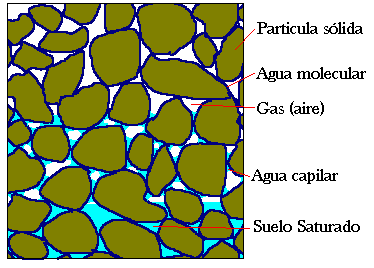
\includegraphics[width=0.5\textwidth]{./img_uf1596/porosidad.PNG}
\caption{\label{fig:org9ca7d26}
Porosidad en suelos}
\end{figure}
\end{center}
El grosor de los poros condiciona la aireación y retención de agua. Los poros
en el suelo se distinguen en \textbf{macroscópicos} y \textbf{microscópicos}.\\
Los terrenos \textbf{arenosos} tienen gran cantidad de poros macroscópicos por lo que tienen una 
muy baja capacidad de retención e agua. Por otro lado los suelos \textbf{arcillosos}
son son ricos en poros microscópicos por lo que tienen una gran capacidad de
retención de agua.
\begin{itemize}
\item \textbf{Densidad:}
\end{itemize}
La relación entre la masa de un suelo y el volumen aparente que ocupa, que
incluye el volumen que ocupan los poros, se denomina densidad aparente.\\
 Es una característica importante de los suelos, puesto que permite conocer su
comportamiento hídrico (capacidad de almacenaje de agua, permeabilidad, etc.) y
sobre su función como hábitat (compactación, facilidad para la penetración de
las raíces´ıces, apertura de galerías, etc.), entre otras.
\begin{itemize}
\item \textbf{Estructura:}
\end{itemize}
La estructura de un suelo es la manera en la que están dispuestos sus
componentes. Las partículas de arena, limo y arcilla se unen entre si de
determinadas maneras formando \uline{terrones}. Según como se unen las partículas y la
forma que adquieren se clasifican en:
\begin{itemize}
\item \textbf{De grano simple:} Frecuente en suelos arenoso ya que los granos
de arena no se unen entre si y se disgregan fácilmente
\item \textbf{Granular:} Frecuente en suelos que ya han sido cultivados. Terrones no muy
grandes y redondeados
\item \textbf{De bloques:} Terrones cuadrados y algo más grandes que la granular
\item \textbf{Prismática:} Terrones más gruesos y alargados
\item \textbf{Laminar:} Muy fácil de identificar por que el suelo está formado por laminas
delgadas horizontales
\item \textbf{Masiva:} En este caso no se forman terrones y el suelo se observa
compacto. Muy común en suelos arcilloso que no han sido cultivados
\end{itemize}
\begin{center}
\begin{figure}[htbp]
\centering
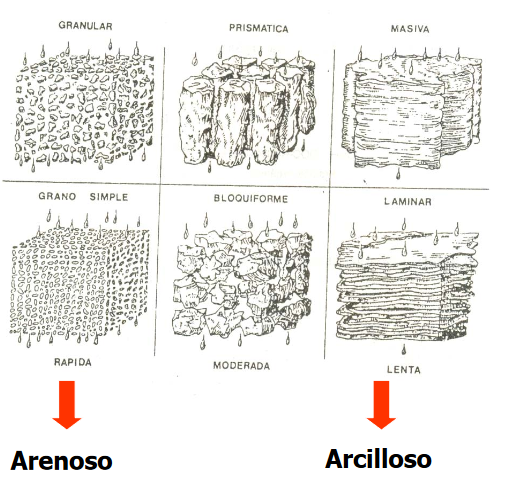
\includegraphics[width=0.65\textwidth]{./img_uf1596/estructura.PNG}
\caption{Principales estructuras en los suelos}
\end{figure}
\end{center}
\subsubsection{Características químicas}
\label{sec:orgf0f2ea7}
La reactividad química de un sustrato se refiere a la transferencia de materia
entre el sustrato y la \uline{solución} nutritiva que alimenta a las plantas a través
de las raíces.

La transferencia puede ser debida a reacciones:
\begin{itemize}
\item \textbf{Químicas}: por la disolución de los nutrientes que lleva el propio sustrato.
\item \textbf{Físico-químicas}: reacciones que se deben a sustratos que tienen
mucha materia orgánica o arcilla
\item \textbf{Bioquímicas}: reacciones que producen la degradación de los materiales que
componen el sustrato. Se origina sobre todo en los materiales de origen
orgánico.
\end{itemize}

Normalmente se \uline{prefieren lo sustratos inertes frente a los químicamente
activos}. La actividad química que se origina en los sustratos puede aportar a
la solución nutritiva \uline{elementos adicionales}, si estos elementos son \uline{tóxicos}
el sustrato no sirve y hay que descartarlo. Pero aunque sean \uline{elementos
nutritivos útiles}  entorpecen el equilibrio de la solución por un aporte extra
con el que hay que contar.
\subsubsection{Características biológicas}
\label{sec:org05b9b56}
Como sabemos la actividad biológica se origina por organismos vivos que
modifican el suelo, insectos, lombrices, hongos, bacterias, algas, etc. A pesar
de que estos organismos vivos son fundamentales para la formación de suelos
\uline{cualquier actividad biológica} en los sustratos es \uline{claramente
perjudicial}. Los microorganismos compiten con las raíces por oxígeno y
nutrientes y también pueden modificar el sustrato empeorando sus características.
\subsection{Preparación del medio de cultivo}
\label{sec:org7f43be8}
En un vivero además de cultivar plantas en macetas, podemos hacerlo en el
suelo, ya sea dentro de los invernaderos o al aire libre. Un factor \uline{fundamental}
para el desarrollo de las plantas son las \uline{condiciones} del suelo, que se mejoran
entre otras técnicas mediante el \uline{laboreo}.
La producción y desarrollo de las plantas está ligada a la \uline{porosidad} del
suelo, ya que son sensibles a la aireación y humedad de su sistema radicular. Es
por lo que el laboreo debe ir dirigido, entre otras cosas, a conseguir una buena
\uline{aireación}, es decir, mejorar la porosidad.
\subsection{Realización de mezclas}
\label{sec:orgdbaf1ab}
En los viveros se producen muchos cultivos en contenedor. Esta manera de
producir plantas tiene unas limitaciones que vienen dadas por el tamaño del
contenedor. El \uline{volumen reducido} de sustrato que hay en un contenedor obliga a
\uline{intensificar el riego}, en comparación con un suelo natural en el que las
plantas pueden desarrollar sus raíces todo lo necesario para buscar agua. Por
tanto los sustratos tendrán como \uline{principal característica} tener una buena
capacidad de \textbf{retención de agua}, pero sin que ello afecte a la \textbf{porosidad} y la
\textbf{densidad}, que como sabemos son factores importantes para el desarrollo de las
raíces y de la planta.
\uline{No se recomienda} el uso de suelo mineral como un componente de sustratos para
macetas, aunque en ciertas circunstancias pueda dar buenos resultados, este tipo
de material tiende a disminuir la porosidad del suelo.
Debe utilizarse una cantidad suficiente de \textbf{componentes orgánicos} en los
sustratos. Este debe haber pasado por un proceso de \textbf{compostaje} para que sea
estable, de esta manera la materia orgánica no se descompondrá mediante
microorganismos que tomarán el nitrógeno del sustrato no dejándolo disponible
para las plantas.
\subsection{Enmiendas y fertilización}
\label{sec:org90838c2}
La mayoría de los componentes orgánicos de un sustrato son ácidos y contienen
\uline{niveles bajos de nutrientes disponibles}. Se recomienda:
\begin{itemize}
\item Aporte de \textbf{cal}: Elevará el pH y además aportará calcio y magnesio que son
\uline{esenciales para el desarrollo radicular}. Estos elementos son retenidos por el
sustrato por lo que no se lavan fácilmente.
\item Para asegurar un buen comienzo del cultivo el nitrógeno (N) debe ser incorporado
antes de plantar. Sin embargo esta práctica es \uline{muy discutible} cuando se usan
fertilizantes inorgánicos (tipo \emph{nitrofoska}) debido al efecto de
contaminación que la \uline{sobre-fertilización} produce en los acuíferos.
\item Fósforo (P) y potasio (K) suelen incorporarse junto al nitrógeno en formulas
N-P-K. El fósforo se \uline{lava menos} mientras que el potasio debería ser
\uline{repuesto periódicamente} ya que no es adsorbido fuertemente por el sustrato.
\item En los suelos calcáreos el hierro (Fe) no esta fácilmente disponible por la
planta debido al pH. La manera más eficiente de aportar este elemento es
mediante \uline{quelato de hierro}, que puede ser absorbida por la planta en un
rango más amplio de pH.
\end{itemize}
\subsection{Desinfección y otros}
\label{sec:orgb2bb180}
Los sustratos pueden estar "contaminados" entre otras cosas de:
\begin{itemize}
\item Semillas de malezas y otras hierbas competidoras
\item Bulbos o rizomas de pastos
\item Larvas de insectos
\item Caracoles o babosas
\item Hongos y patógenos
\item Nemátodos
\end{itemize}
Es muy importante que los sustratos estén debidamente desinfectados. Mencionamos
algunas medidas:
\begin{itemize}
\item \textbf{Cribar} el sustrato para retener partículas grandes de vegetales, insectos u
otros organismos
\item \textbf{Solarización:} Disponer el sustrato en camas, humedecerlo hasta saturación y
después cubrirlo con plástico negro o transparente. Se deja expuesto al sol y
las variaciones de calor causan la muerte de los microorganismos patógenos.
\item \textbf{Fitotipren:} mezcla de varios hongos para el control de enfermedades como
\emph{Fusarium, Rhizoctonia, Pytium}.
\item \textbf{Rutinal (extracto de ruda \emph{Ruta graveolens}):} para control de nemátodos y
desinfectante natural de suelos.
\item \textbf{Botrycid:} para control de \emph{Rhizoctonia} y \emph{Fusarium}. Es muy eficiente
controlando bacterias como \emph{Erwinia, Xanthomonas, Agrobacterium} y \emph{Pseudomonas}.
\item \textbf{Anisafer:} para el control de chizas, gusanos tirreros, picudos, chinches y
hormiga arriera.
\end{itemize}
\subsection{Equipos y maquinaria}
\label{sec:orgd2d5db5}
Todas las labores que se han comentado se pueden mecanizar. Existen máquinas de
todo tipo y para todas las operaciones. A continuación vamos a ver las más
habituales en elaboración de medios de cultivo en vivero.
\begin{itemize}
\item \textbf{Descompactadora de turba} de \emph{big balé} (gran paca o gran fardo)
\end{itemize}
\begin{center}
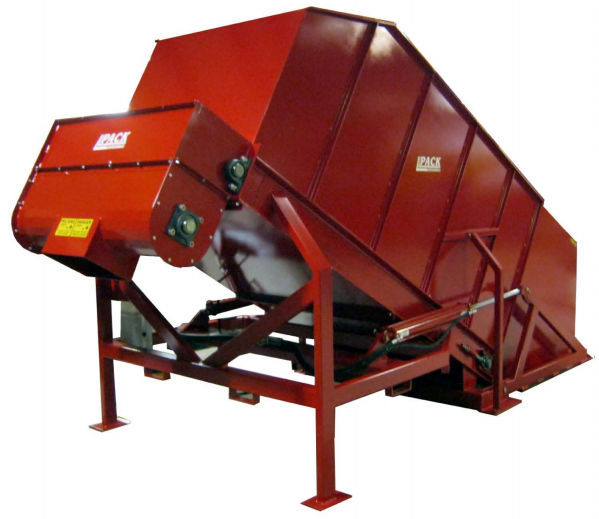
\includegraphics[width=0.4\textwidth]{./img_uf1596/big_bale.jpg}
\end{center}
\begin{itemize}
\item \textbf{Mezcladora}
\end{itemize}
\begin{center}
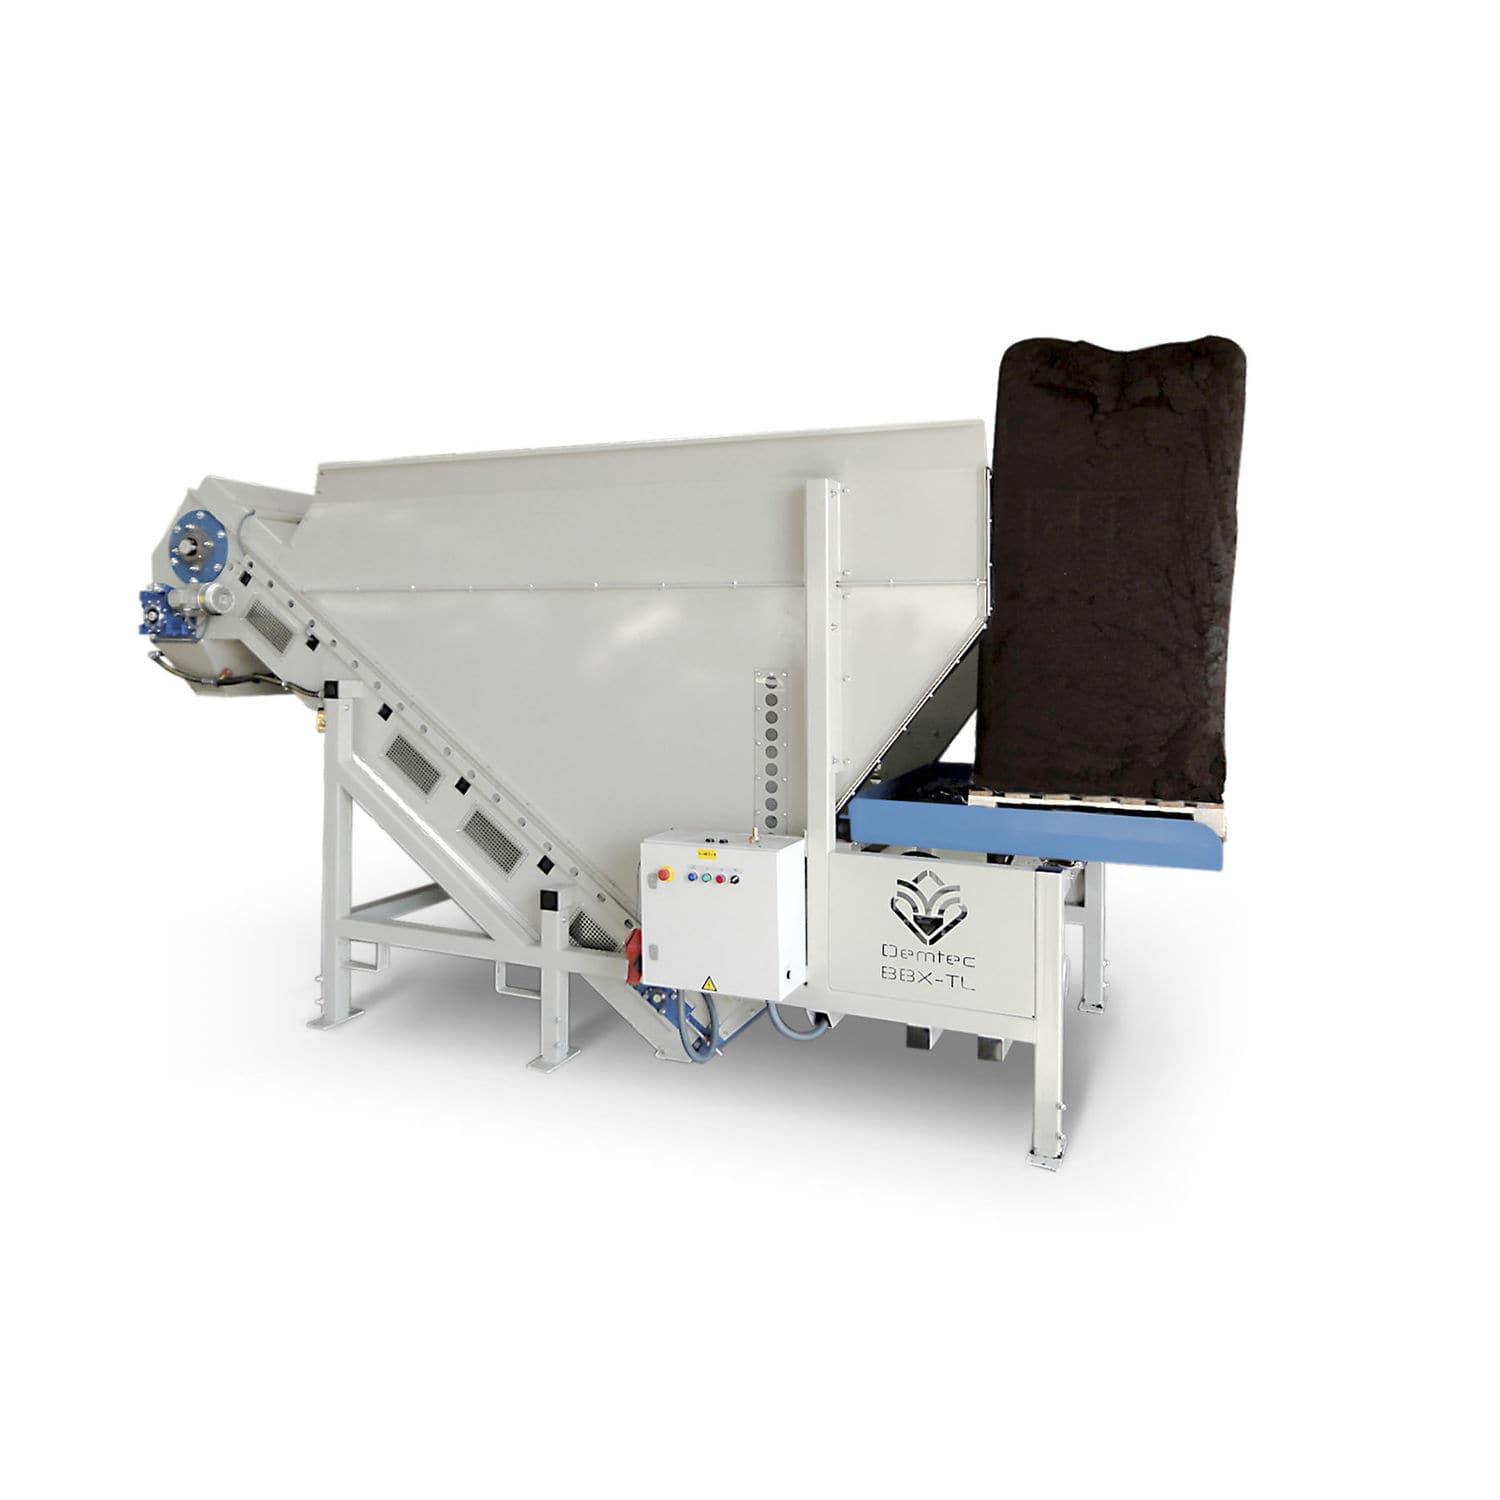
\includegraphics[width=0.5\textwidth]{./img_uf1596/mezcladora.jpg}
\end{center}
\begin{itemize}
\item \textbf{Mezcladora y llenadora de bandejas}
\end{itemize}
\begin{center}
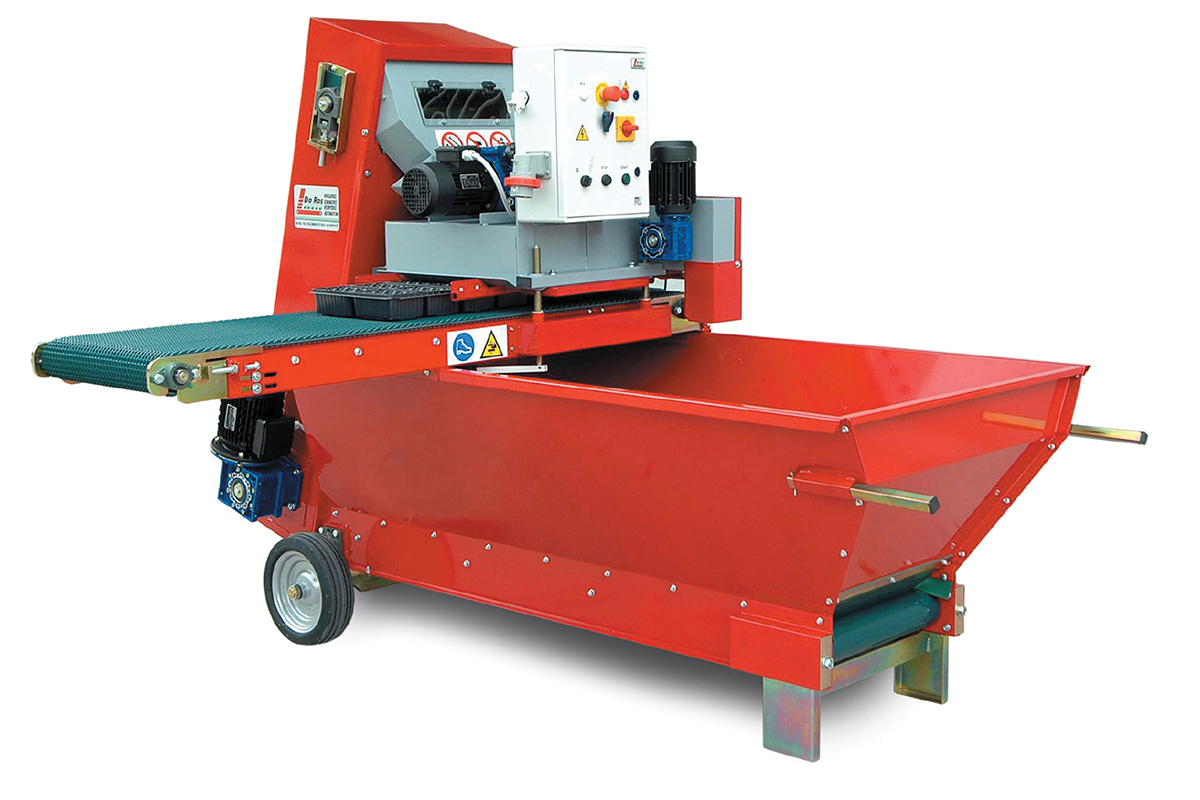
\includegraphics[width=0.5\textwidth]{./img_uf1596/bandejas_mezcladora.jpg}
\end{center} 
\begin{itemize}
\item \textbf{Enmacetadora}
\end{itemize}
\begin{center}
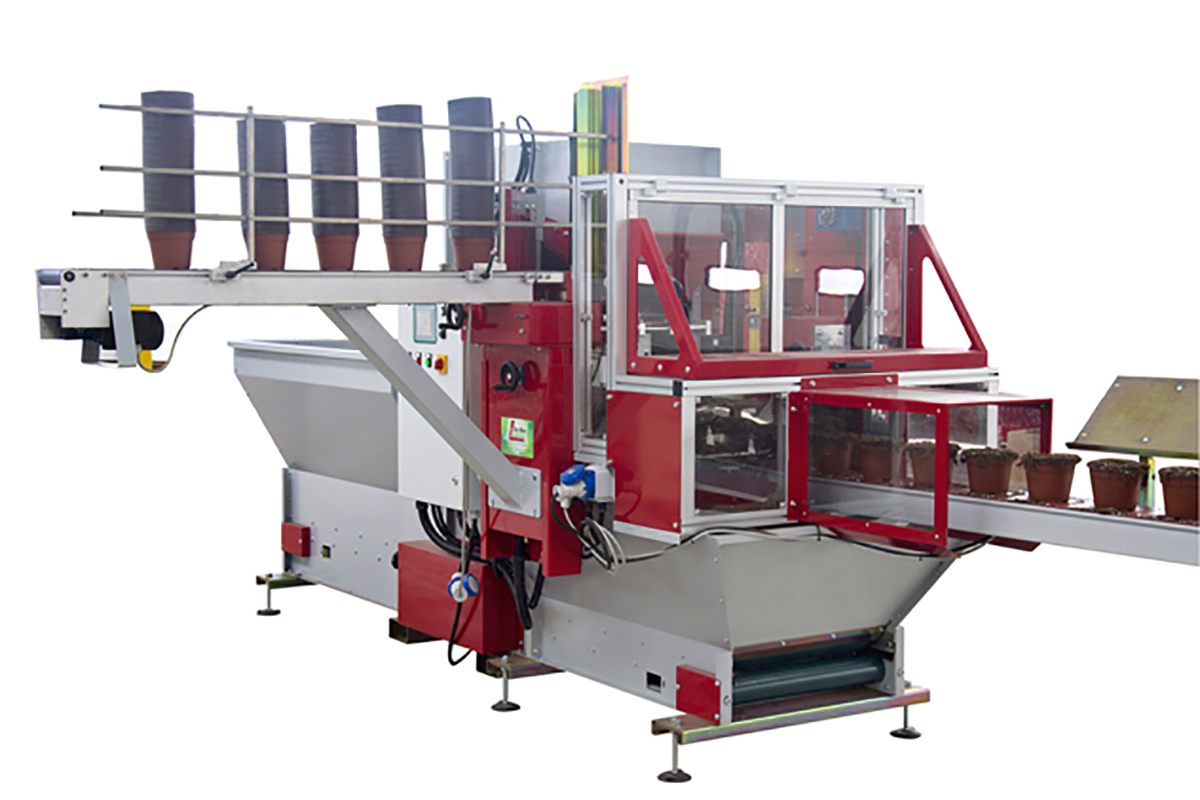
\includegraphics[width=0.5\textwidth]{./img_uf1596/enmacetadora.jpg}
\end{center}
\begin{itemize}
\item \textbf{Transplantadora de bandejas}
\end{itemize}
\begin{center}
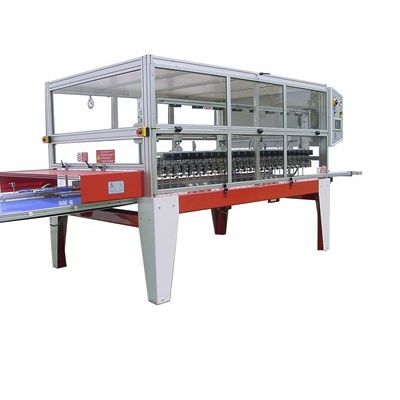
\includegraphics[width=0.5\textwidth]{./img_uf1596/transplantadora_bandejas.jpg}
\end{center}
\begin{itemize}
\item \textbf{Sembradora de líneas}
\end{itemize}
\begin{center}
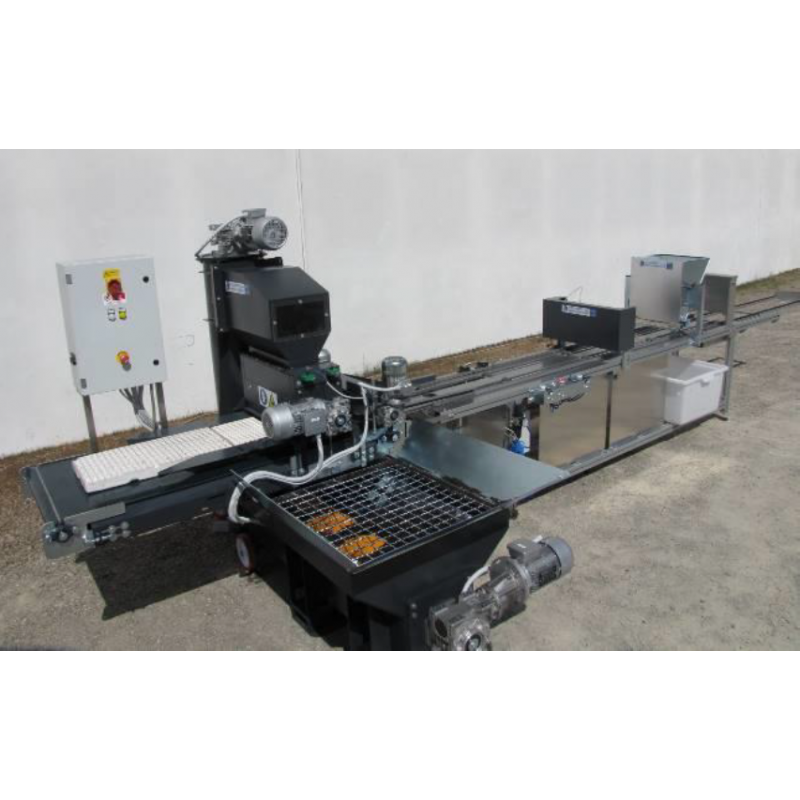
\includegraphics[width=0.5\textwidth]{./img_uf1596/sembradora_bandejas.png}
\end{center}
\section{Trasplante de plantas}
\label{sec:org26acf47}
\subsection{Introducción}
\label{sec:orge911bef}
El trasplante consiste en trasladar una planta de una maceta a otra más grande
o al terreno definitivo.

Para realizar el trasplante hay que \uline{tener en cuenta muchos factores}, por lo
que \uline{no se pueden} dar unas pautas fijas de cuando y como. Pero \uline{si se puede}
dar \textbf{una norma clara y concisa}:
\begin{center}
\textbf{El trasplante se realiza cuando la planta ha llenado con raíces todo el
 contenedor} 
\end{center}
\subsection{Estadios de desarrollo del cultivo}
\label{sec:org2c39632}
Las plantas que hay que trasplantar pueden proceder de:
\begin{itemize}
\item Multiplicación vegetativa, \uline{generalmente esquejes}. Podemos encontrar los
siguientes \_tipos de esquejes:
\begin{itemize}
\item Esquejes herbáceos: clavel, crisantemo, salvia
\item Esquejes de madera blanda o semi verde: Aquellos tallos que no han comenzado
a lignificarse.
\item Esquejes de madera semi dura: el tallo ha comenzado el proceso de
lignificación pero no es leñoso del todo. Se emplea para especies arbustivas
sobre todo
\begin{itemize}
\item Boj (Buxus sempervirens)
\item Callistemon (Callistemon rigidus)
\item Adelfa (Nerium olenader)
\item Pitosporo (Pittosporum tobira)
\end{itemize}
\item Esquejes de madera dura de especies perennes
\begin{itemize}
\item Árbol de Júpiter (Lagerstroemia indica)
\item Hibisco (Hibiscus siryacus)
\item Rosal (Rosa spp.)
\end{itemize}
\item Especies de madera dura de especies caducas
\begin{itemize}
\item Higuera (Ficus carica)
\item Chopo (Popoulus spp.)
\item Ginkgo (Ginkgo biloba)
\item Agracejo (Berberis spp.)
\end{itemize}
\end{itemize}
\item Multiplicación por semillas o sexual
\end{itemize}

El \uline{enraizamiento} de los esquejes se inicia en unas condiciones óptimas de
\uline{humedad y temperatura}. Consideramos que está suficientemente desarrollado
cuando se puede extraer con el esqueje \uline{todo el cepellón} con facilidad.

Las plantas que proceden de semilla \uline{estarán preparadas} para el trasplante al
igual que los esquejes, cuando las raíces se han desarrollado \uline{suficientemente}
por ido el alveolo y podemos extraer el cepellón con facilidad. 

\uline{El tiempo} que debe transcurrir para la \uline{germinación} varía mucho de unas
especies a otras. Cambia en función de \uline{condiciones de cultivo} como son
\uline{temperatura, luminosidad, medio de cultivo, humedad ambiental}, etc
\subsection{Operaciones pre-trasplante.}
\label{sec:org6f38e8d}
\subsubsection{Endurecimiento}
\label{sec:orgbb2d474}
Consiste en someter a las plántalas a una serie de \uline{condiciones ambientales
adversas} para que resistan  mejor el trasplante.

Con el  endurecimiento conseguimos que la planta \uline{detenga o disminuya el
crecimiento de la parte aérea} y de esta manera favorecemos que \uline{se desarrolle
el sistema radicular}, y la acumulación de sustancias de reserva. 

Podemos conseguir el endurecimiento de tres formas:
\begin{itemize}
\item Por bajas temperaturas
\item Por estrés hídrico
\item Por falta de determinados nutrientes como nitrógeno (N) y potasio (K)
\end{itemize}

Cuando se realiza el endurecimiento \uline{hay que tener muy caen cuenta} las
condiciones en las que están las plantas y las condiciones que tendrán que
soportar en el trasplante
\subsubsection{Recepción del material}
\label{sec:orgef416d6}
Puede que las plantas las hayamos producido nosotros o vengan de otro
vivero. En cualquier caso \uline{hay que prestar atención al estado en que nos
llegan} antes de proceder a su trasplante.
\begin{enumerate}
\item \textbf{Algunas recomendaciones para el descarte de plantas:}
\begin{itemize}
\item En primer lugar descartaremos las que tengan \uline{signos de enfermedades o ataques}
de plagas, las débiles, las que tengan heridas y las deformes.
\item Las plantas \uline{vivaces} han de tener buen aspecto. Descartaremos las raquíticas
o envejecidas, con tallo pelado y las que tengan flores \uline{solo en su parte más
alta}
\end{itemize}
\item \textbf{Recomendaciones para la revisión general de plantas:}
\begin{itemize}
\item \uline{Regar los semilleros} para poder extraer fácilmente el cepellón \uline{sin dañar
las raíces}
\item Trasplantar las que tengan un aspecto \uline{sano, con hojas bien desarrolladas
y buen color}
\item Las plantas \uline{deben tener} un sistema radicular \uline{bien desarrollado}, con
raíces \uline{blancas y delgadas}. La presencia de \uline{raíces marrones} son señal de
exceso de humedad o problemas de pudriciones radicales
\end{itemize}
\end{enumerate}
\subsection{Tipos de contenedores}
\label{sec:org79ecbc9}
Los contenedores son muy importantes ya que son el suelo de las
plantas. Cualquier recipiente puede ser utilizado como maceta para mantener una
planta, pero para a \uline{producción de planta los contenedores deben satisfacer
otras necesidades}.
\subsubsection{Cualidades de los contenedores para producción de planta}
\label{sec:org8bc70fc}
\begin{itemize}
\item Ante todo ser \textbf{funcional} y permitir la \textbf{mecanización} (llenado y semillado
por ejemplo)
\item \textbf{Manejable} y \textbf{Resistente}
\item Ocupar mínimo \textbf{espacio}
\item Que se pueda \textbf{agrupar} en bandejas y/o apilar
\item Que se pueda reciclar (utilizar varias veces)
\end{itemize}
\subsubsection{Materiales}
\label{sec:org98bfecc}
A continuación describimos los principales materiales empleados en la
fabricación de contenedores para producción de planta.\\
\begin{enumerate}
\item Macetas biodegradables
\label{sec:org092f01c}

Macetas fabricadas a base de fibras vegetales. La característica más
interesante es que la planta que se ha desarrollado en estas macetas \uline{no
necesita trasplante}: se puede introducir directamente dentro de un a maceta o
en el suelo \uline{sin necesidad de sacarla del contenedor}. Una vez la maceta
plantada, esta se degrada rápidamente y se transforma en materia orgánica.

En el cultivo en maceta biodegradable, la planta al crecer, atraviesa muy
fácil mete las paredes de la maceta. Esto no pasa con otro tipo de contenedor,
como por ejemplo las macetas de plástico. Al entrar en contacto con el aire las
raíces \uline{detienen su crecimiento}. Esto estimula la creación de raíces
secundarias que ocupan el volumen de la maceta. Este fenómeno se llama ``poda
aérea radicular'' y resulta muy beneficioso tanto para el productor como el
cliente.
\item Barro cocido
\label{sec:orgdb12862}

Los contenedores de barro cocido tienen las siguientes características:
\begin{itemize}
\item Suelen ser \uline{pesados}. Lo que los hace muy estables pero poco manejables
\item Resisten heladas suaves siempre que estén secos
\item Existen macetas de \uline{terracota}, que resisten las heladas y permiten respirar a
las raíces al ser más porosas
\end{itemize}
\item Plástico
\label{sec:org4fb5df4}

Son \uline{muy ligeros} lo que los hace \uline{manejables, duraderos y baratos}. Tienen las
\uline{desventajas} de que se rajan con facilidad y que dañan las raíces cuando se
calientan demasiado. 

En la mayoría de los casos no cuentan con sistemas \uline{antiespiralizantes}. Esto
puede dificultar el enraizamiento posterior de la planta ya que si la raíz se ha
desarrollado de esta manera, tenderá a seguir una disposición en espiral cuando
se trasplante.

Diferenciamos contenedores de plástico según su uso:
\begin{enumerate}
\item \textbf{Para semilleros:}
\begin{itemize}
\item Bandejas de semillero o cubetas: Son las empleadas para \uline{semillas con un
porcentaje de germinación muy bajo}. Las bandejas de semillero \uline{obligan al
repicado a raíz desnuda}
\item Bandejas mini-alveolares: cuentan con un gran número de alveolos de muy
pequeño volumen. Se recomiendan para semillas con porcentajes de
germinación medios o altos. No se emplean si el porcentaje de germinación
es muy bajo.
\begin{center}
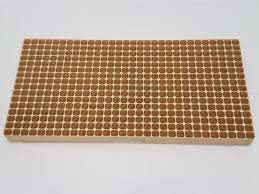
\includegraphics[width=0.5\textwidth]{./img_uf1596/bandeja_multi.jpg}
\end{center}
\item Bandejas de alvéolos: Tienen volúmenes comprendidos entre 150 y 350 cm\(^{\text{3}}\) y
se emplean para semillas con porcentajes altos. Se pueden emplear para
semillas grandes como \uline{bellotas, castañas o cicas} que se quieren dejar
todo el primer año y no hay que repicarlas o trasplantarlas (arboles para
engorde y planta forestal para repoblaciones)
\end{itemize}
\item \textbf{Para el estaquillado:} Encontramos los mismos sistemas que para semillado
pero \uline{sin utilizar bandejas de semillero}
\begin{itemize}
\item Bandejas de mini-alvéolos: para estaquillados de muy pequeño tamaño, como
los de \uline{aromáticas}
\item Bandejas de alvéolos de pequeño tamaño (75-150cm\(^{\text{3}}\)): para el estaquillado
semileñoso y leñoso. La estaquilla estará hasta que enraíce y se
trasplantará a contenedor individual para el engorde
\item Bandejas de alvéolos de mayor volumen (200-300 cm\(^{\text{3}}\)): Normalmente solo se
utilizan en viveros forestales
\end{itemize}
\item \textbf{Para el engorde:}
\begin{itemize}
\item De plástico y sin sistema antiespiralizante: En el caso de tener a la venta planta
pequeña, generalmente se emplean contenedores de sección cuadrados que
aprovechan el espacio mejor que los circulares.
\begin{center}
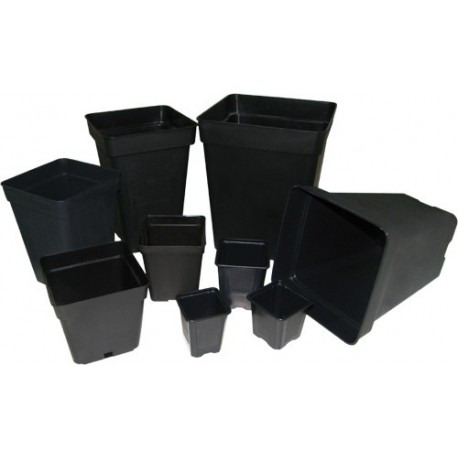
\includegraphics[width=.9\linewidth]{./img_uf1596/maceta_cuadrada.jpg}
\end{center}
\item Con sistema antiespiralizante: Son más caros que los anteriores. También
tiene mayor volumen. Encarece el coste de la planta pero crean un sistema
radicular más equilibrado.
\item Contenedores de metal: Se usan mucho como grandes contenedores
\uline{decorativos} en calles y plazas públicas
\item Contenedores de papel: Muy usados en plantación de hortalizas, ya que sus
paredes son atravesadas fácilmente por las raíces
\item Otros materiales: Vidrio, cemento, hormigón, fibra de vidrio, etc.
\end{itemize}
\end{enumerate}
<<<<<<< HEAD
\end{enumerate}
\subsection{Técnicas de trasplante}
\label{sec:orgb31d39a}
\texttt{=====}
\subsection{Técnicas de trasplantes}
\label{sec:org25983a4}
En ocasiones cuando la planta va desde un contenedor a otro se le llama
también repicado. El trasplante propiamente dicho, sería cuando pasamos las
plantas a un lugar definitivo. Nosotros definiremos el trasplante como \uline{el
traslado de la planta de un lugar a otro}.

\subsubsection{La raíz de la planta.}
\label{sec:orgd0d2031}
Cuando producimos planta, tenemos que elegir un sistema de trasplante, esto es
a raíz desnuda o en contenedor

\begin{enumerate}
\item A raíz desnuda
\label{sec:org53de76b}

Encontramos las siguientes ventajas e inconvenientes
\begin{itemize}
\item Ventajas:\\
\begin{itemize}
\item \uline{Menor coste de producción}
\item Podemos hacer los semilleros en camas sobre el suelo por lo que \uline{ahorramos
espacio}
\item Si el trasplante se retrasa las plantas aguantan más a raíz desnuda
\end{itemize}
\item Inconvenientes:\\
\begin{itemize}
\item El estrés que sufre la planta en el trasplante es mucho mayor que con
cepellón. Se rompen muchas raíces al arrancar las plantas del suelo y la
planta tarda más tiempo en desarrollarse
\item En el semillero a raíz desnuda es difícil conseguir homogeneidad en las plantas
\item Si las \uline{condiciones ambientales} son desfavorables el día del trasplante,
tendremos una \uline{mayor probabilidad de marras}
\end{itemize}
\end{itemize}

\item Con cepellón
\label{sec:org7282be6}

\begin{itemize}
\item Ventajas:\\
\begin{itemize}
\item El trasplante con cepellón \uline{reduce el estrés al mínimo}
\item El primer riego \uline{no es tan importante} ya que las plantas tienen su
\uline{sistema radicular intacto}
\item Al estar cada planta en su contenedor hay \uline{menor riesgo de propagación de
enfermedades}
\end{itemize}
\item Inconvenientes:\\
\begin{itemize}
\item \uline{Mayor coste} de producción.
\item Las plantas tienen \uline{un espacio determinado para crecer} por lo que hay que
\uline{trasplantar} ya que si no se hace a tiempo las plantas podrían sufrir
daños
\end{itemize}
\end{itemize}
\end{enumerate}

\subsubsection{Destino de la planta}
\label{sec:org210f893}
Cuando trasplantamos planta tenemos dos opciones, trasplantar a un contenedor
o trasplantar en suelo. 

\begin{enumerate}
\item Destino a contenedor:
\label{sec:org83fa97b}

Lo más importante es \uline{saber elegir el contenedor adecuado} ya que una mala
elección puede suponer un gasto extra que seria innecesario. Veamos dos ejemplos.
\begin{itemize}
\item Contenedor \uline{mayor de lo necesario}:
\begin{itemize}
\item Mayor coste en sustrato
\item Mayor peso y volumen para transportes y almacenamientos
\item Mayor gasto de agua y costes de mantenimiento
\end{itemize}
\item Contenedor más \uline{pequeño de lo necesario}:
\begin{itemize}
\item Posible problemas de \uline{desarrollo de las raíces} por falta de espacio.
\end{itemize}
\end{itemize}

\item Destino a suelo:
\label{sec:org730194e}

El trasplante a suelo se realiza con árboles, hortícolas, arbustos, y en el
ajardinamiento de nuevas zonas o mantenimiento de jardines.

En el caso de las \uline{hortícolas} el trasplante está muy mecanizado 
\begin{figure}[htbp]
\centering
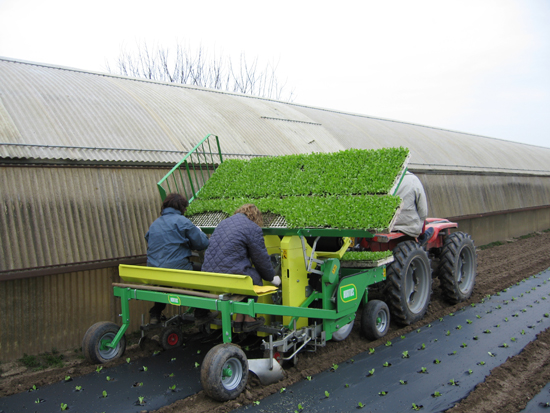
\includegraphics[width=0.5\textwidth]{./img_uf1596/transplantadora_suelo.jpg}
\caption{Transplantadora automática}
\end{figure}

Para el resto de plantas, árboles y arbustos vamos a ver unas serie de \uline{normas
básicas}:
\begin{itemize}
\item No extender nunca los plantones por la parcela. \uline{Se deben extender a medida se
plantan}. De esta manera evitaremos la \uline{deshidratación}
\item Deshacer \uline{suavemente} el cepellón antes de plantar
\item \uline{Repartir} las raíces en el hoyo de plantación
\item \uline{Cortar las raíces en mal estado} ya que pueden ser la \uline{entrada de hongos y
enfermedades}
\item \uline{No aplicar} abonos minerales ni estiércol en el hoyo de plantación
\item Muy importante el \uline{riego de plantación}
\item Elegir la fecha de plantación en la medida de lo posible teniendo en cuenta:
\begin{itemize}
\item Ciclo biológico de la planta
\item Condiciones meteorológicas
\end{itemize}
\end{itemize}

\begin{enumerate}
\item Trasplante de grandes árboles
\label{sec:org4658314}

Para el trasplante de grandes árboles que están plantados en suelo se puede
emplear la técnica del \uline{escayolado}.

Esta técnica consiste en preparar un recipiente a medida del sistema radicular y
envolverlo con malla metálica y escayola a modo de gran maceta y con un cepellón
adecuado a su tamaño. El cepellón debe tener por su parte inferior agujeros para
facilitar el drenaje. 
\begin{figure}[htbp]
\centering
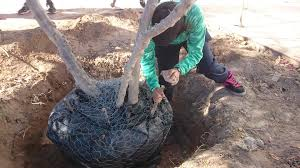
\includegraphics[width=0.5\textwidth]{./img_uf1596/escayolado_1.jpg}
\caption{Preparación del cepellón y colocación de malla metálica}
\end{figure}
\begin{figure}[htbp]
\centering
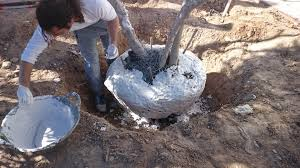
\includegraphics[width=0.5\textwidth]{./img_uf1596/escayolado_2.jpg}
\caption{Aplicación de la escayola}
\end{figure}
\begin{figure}[htbp]
\centering
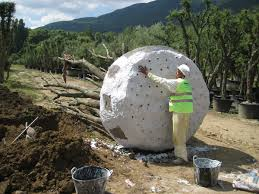
\includegraphics[width=0.5\textwidth]{./img_uf1596/escayolado_3.jpg}
\caption{Escayolado en árbol de grandes dimensiones}
\end{figure}]]

Los árboles se plantan en el nuevo hoyo con la escayola ya que con el tiempo
esta se va deshaciendo.

Existen también máquinas que extraen los árboles del suelo con un buen número de
raíces  

\begin{figure}[htbp]
\centering
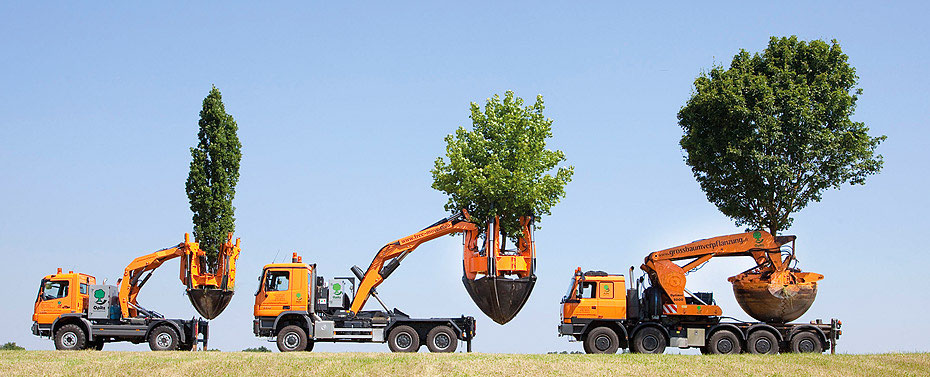
\includegraphics[width=0.5\textwidth]{./img_uf1596/arbol_transplante_maquina.jpg}
\caption{Árbol extraído por máquina especializada}
\end{figure}
\end{enumerate}
\end{enumerate}

\subsubsection{Formas de trasplante}
\label{sec:org487235b}

\begin{enumerate}
\item Trasplante mecanizado
\label{sec:orgc5e03bd}

Se realiza con distintas máquinas. A continuación mencionamos brevemente algunas
de las que hay en el mercado

\begin{enumerate}
\item Robot de trasplante bandeja a bandeja
\label{sec:org9867a60}
Las plantas llegan por     
\item Robot de trasplante sobre máquina enmacetadora
\label{sec:orgb4e2934}
Coge las plantas directamente sobre bandejas y las coloca sobre la máquina enmacetadora. Puede tener un rendimiento de entre 5000 y 6000 plantas por hora.
\item Transplantadora semiautomática
\label{sec:orga06b248}
Para plántulas de cepellón cónico y piramidal. Se acciona por ruedas compactadoras posteriores. Hay diferentes modelos. En algunos las plántulas las introduce el operario en un sistema de distribución giratorio. Se puede regular la distancia entre líneas y entre plantas. El rendimiento puede variar entre 3000 y 7000 plantas por línea y por hora
\end{enumerate}
\item trasplante manual
\label{sec:orgc37d7d3}

Como hemos visto se puede realizar con plantas a raíz desnuda o con cepellón.
\end{enumerate}
\end{document}